\documentclass[10pt,twocolumn]{article}
\usepackage[margin=0.75in]{geometry}
\usepackage{times}
\usepackage{microtype}
\usepackage{graphicx}
\usepackage{booktabs}
\usepackage{amsmath, amssymb}
\usepackage{siunitx}
\usepackage{hyperref}
\usepackage{cleveref}
\usepackage[numbers]{natbib}
\usepackage[utf8]{inputenc}
\usepackage[font=small,labelfont=small]{caption}

% Macros
\newcommand{\rmse}{\ensuremath{\mathrm{RMSE}}}
\newcommand{\rTwo}{\ensuremath{\mathrm{R}^2}}
\newcommand{\da}{\ensuremath{\mathrm{DA}}}

% Custom title formatting
\makeatletter
\renewcommand{\@maketitle}{%
  \newpage
  \null
  \vskip 2em%
  \begin{center}%
  \let \footnote \thanks
    {\Huge \@title \par}%
    \vskip 1.5em%
    {\large
      \lineskip .5em%
      \begin{tabular}[t]{c}%
        \@author
      \end{tabular}\par}%
    \vskip 1em%
    {\large \@date}%
  \end{center}%
  \par
  \vskip 1.5em}
\makeatother

% Metadata
\title{Comparing Transformer and Baseline Models for Multi-Horizon Stock Return Prediction with Technical and Event Features}

\author{Nelson Siu \\
\textit{Division of Engineering Science} \\
\textit{University of Toronto} \\
nelson.siu@mail.utoronto.ca
\and
Jonathan H. Chan \\
\textit{Innovative Cognitive Computing} \\
\textit{King Mongkut's University of Technology Thonburi} \\
jonathan@sit.kmutt.ac.th}

\date{}

\begin{document}
\maketitle

\begin{abstract}
We study daily multi-horizon equity return prediction on the Dow 30 with horizons $h\in\{1,5,21\}$ using technical indicators and earnings features. We compare models across sequence (GRU, LSTM), transformer (TFT), and tabular (Ridge, Random Forest, XGBoost) classes under a strict temporal split. At $h=1$, LSTM attains the lowest \rmse{} (0.01622), 0.8--1.5\% below the strongest tabular baselines and essentially tied with GRU (0.17\% difference). At $h=5$, Ridge achieves the best \rmse{} (0.03651), 4--8\% lower than tree ensembles and $\sim$37\% lower than deep sequence/transformer models. At $h=21$, LSTM's \rmse{} (0.05084) is within 0.03--0.24\% of GRU/TFT yet 31--38\% below tabular baselines; it also yields the best \da{} (55.0\%), beating GRU/TFT by $\sim$1.1 pp and tabular models by 0.8--3.4 pp. All \rTwo{} values are $\sim$0 or slightly negative because the benchmark is a zero-return predictor; this is typical for daily returns and makes directional accuracy the more discriminative metric here. Regime slices at $h=21$ show GRU lowest \rmse{} in the 2022 bear and LSTM lowest \rmse{} in the 2023--24 rally, while \da{} is highest around earnings windows (61.4\% vs. 53.9\% otherwise). Overall, simple sequence models are competitive on daily panels, while tabular baselines remain strong on \rmse{} at intermediate horizons.
\end{abstract}

\section{Introduction}
Multi-horizon equity prediction remains challenging given noisy targets, regime dependence, and the potential for only small predictive signals. We present a clear, apples-to-apples comparison across model classes on the Dow 30 with realistic event sensitivity, evaluating how different modeling approaches perform under consistent data splits and feature sets.

\textbf{Contributions.}
\begin{itemize}
    \item \textit{Robust experimental design:} Strict, reproducible temporal split (2016--2019 train, 2020 val, 2021--2024 test) and Dow 30 constituents fixed as of 2018-01-01 to mitigate survivorship bias.
    \item \textit{Model class comparison:} Compare sequence/transformer vs. tabular models on identical technical + earnings feature sets.
    \item \textit{Comprehensive evaluation:} Evaluate \rmse{}, \rTwo{}, and \da{} across $h\in\{1,5,21\}$, plus detailed regime (bear vs. rally) and earnings window slices.
    \item \textit{Insights:} Identify where each model class wins (e.g. bear vs. rally regimes; around earnings windows) and discuss why simpler models can rival more complex ones on daily financial data.
\end{itemize}

\subsection*{Hypotheses}

\textbf{H1 (Model class advantage).} Given multi-horizon forecasting with technical and earnings features on a pooled Dow 30 panel, the Temporal Fusion Transformer (TFT) will achieve lower \rmse{} and higher \da{} than strong baselines (LSTM, GRU, XGBoost, Random Forest, Ridge) on the 21-day horizon.

\textbf{H2 (Event features add value).} Adding earnings/event features to technical indicators will improve \da{} (and not worsen \rmse{}) relative to technical-only inputs at the 21-day horizon.

\textbf{H3 (Regime dependence).} Model rankings differ by market regime: sequence models (LSTM/GRU) will outperform tabular and transformer models during trending rally periods, while performance gaps will narrow or reverse during bear markets.

\paragraph{Decision criteria.}
We evaluate each hypothesis using the held-out test set (2021--2024) across three random seeds:
\begin{itemize}
  \item \textit{H1:} TFT beats the best non-TFT model at $h{=}21$ by (i) a statistically significant Diebold--Mariano test on squared error (p{<}0.05) and/or (ii) a McNemar or paired test on directional hits (p{<}0.05), with effect sizes of at least $\geq$2\,pp in \da{} or $\geq$5\% relative improvement in \rmse{}.
  \item \textit{H2:} Tech{+}Earnings vs Tech-only shows \da{} $\uparrow$ ($\geq$2\,pp) and \rmse{} $\not\uparrow$ (95\% CI overlap) for at least one strong model (e.g., TFT or XGBoost) at $h{=}21$.
  \item \textit{H3:} Best-in-class models differ across regimes (2022 bear vs 2023--24 rally), verified by per-regime leaderboards and non-overlapping bootstrap CIs.
\end{itemize}

\paragraph{Hypothesis rationale.}
H1 reflects a common prior that attention-based architectures should capture long-range dependencies and heterogeneous covariates better than simpler sequence/tabular models \citep{lim2021temporal}, potentially yielding gains at longer horizons (here, $h{=}21$). H2 follows established finance findings that earnings-related variables (surprises, timing) add predictive power, particularly over weeks due to PEAD \citep{bernard1989,schnaubelt2020}. H3 is motivated by the Adaptive Markets Hypothesis \citep{lo2004} and regime-dependent performance noted in recent reviews (e.g., pre-/post-COVID comparisons) \citep{zhang2023review}. Our decision thresholds (2 pp in \da{}, 5\% in \rmse{}) target effects that are practically meaningful given typical daily-return noise and avoid declaring wins on statistically significant but economically negligible differences.

\paragraph{Outcome transparency.}
H1 specifically tests TFT on \emph{technical+earnings} inputs; H2 is a clean test of event-feature value.

\section{Related Work}
Classical and modern approaches have been explored for multi-horizon financial forecasting (1-day, 1-week, 1-month), with varying success across horizons and regimes.

\paragraph{Classical time-series baselines.} ARIMA-family models remain common reference points but rely on linearity and (quasi-)stationarity that degrade at longer horizons and across regime shifts \citep{box2015}. VAR extensions inherit similar limitations in high-dimensional, nonstationary settings. GARCH-style volatility models are informative for conditional variance rather than mean return; as such, their direct use for multi-step return prediction is limited relative to modern ML baselines.

\paragraph{Traditional ML baselines and horizon effects.} Tree ensembles and SVMs often improve over linear models when fed engineered features, yet accuracy typically decays with horizon length due to error accumulation \citep[][and references therein]{gu2018,chen2016xgboost}. Recent surveys report multi-horizon degradation patterns (e.g., 1-day to 20-day) in a variety of assets and markets \citep{zhang2023review}. In stock panels, ML methods materially outperform simple linear rules on cross-sectional tasks, though absolute gains can be modest and sensitive to validation protocols \citep{gu2018}.

\paragraph{Deep and hybrid architectures.} Recurrent neural networks (LSTM and GRU) capture sequential dependencies and have outperformed classical and tree models in several studies \citep{hochreiter1997long,cho2014learning,fischer2018,selvin2017}. Hybrids such as CNN-LSTM can improve short- and longer-horizon accuracy by extracting local patterns before temporal aggregation \citep{selvin2017}. Echo State Networks (ESN) provide efficient sequence modeling with reservoir dynamics and have been explored in financial forecasting \citep{jaeger2001esn}.

\paragraph{Attention and transformers for multi-horizon.} Attention mechanisms help models focus on horizon-specific context; attention-based CNN-LSTMs have been used for crypto markets \citep{xu2022bitcoin}. The Temporal Fusion Transformer (TFT) \citep{lim2021temporal} directly targets multi-horizon outputs by combining recurrent encoders with static/contextual encoders and interpretable attention. In finance and crypto applications, TFT variants have been reported to capture both short- and long-range relationships; however, controlled, apples-to-apples evaluations on small daily panels often find transformers comparable to strong RNN baselines, reinforcing the need for rigorous study designs \citep{zhang2023review}.

\paragraph{Hybrid and ensemble methods.} Combining linear and nonlinear components can mitigate misspecification: exponential-smoothing/RNN hybrids and ARIMA-LSTM variants have yielded competitive results in forecasting competitions and financial applications \citep{smyl2020}. Practitioners also combine deep sequential encoders with tabular learners to exploit complementary biases. In equity cross-sections, ensembles of boosted trees, random forests, and deep nets remain strong \citep{krauss2017}.

\paragraph{Integrating technical, earnings, and events.} Beyond technical indicators, structured earnings/event features carry predictive power, consistent with post-earnings-announcement drift (PEAD) \citep{bernard1989}. Earnings and revenue surprises rank highly among predictive covariates at weekly-to-monthly horizons \citep{schnaubelt2020}. Richer fusion of prices, events, and news (e.g., knowledge graphs) further improves performance while aiding interpretability \citep{cheng2022}. Our study sits in this line by emphasizing earnings/event features alongside technicals under strict temporal evaluation.

\paragraph{Regimes and evaluation design.} Model efficacy varies with market conditions per the Adaptive Markets Hypothesis \citep{lo2004}. Empirically, performance differs between pre-COVID, COVID, and post-COVID regimes and across horizons \citep{zhang2023review}. These observations motivate regime-aware evaluation and horizon-specific metrics, which we adopt in our experimental design.

\paragraph{Gaps and contributions.} Despite progress, gaps remain: rigorous apples-to-apples comparisons of RNNs, transformers, and tabular models on identical feature sets are rare; structured earnings/event features are underused in deep forecasting; and evaluation protocols sometimes risk look-ahead bias. Our study addresses these by (i) directly comparing RNNs, TFT, and tabular models on the same Dow 30 panel, (ii) incorporating technical plus earnings/event features to quantify additive value, and (iii) using strict temporal splits with regime- and event-based slices for robust assessment.



\section{Data \& Experimental Design}
\textbf{Universe.} The Dow 30 stock universe is frozen as of \texttt{2018-01-01} (see Appendix A for constituents) to mitigate survivorship bias.

\textbf{Splits.} We use a strict temporal split: Train set spans \texttt{2016-01-01} to \texttt{2019-12-31}; Validation is \texttt{2020-01-01} to \texttt{2020-12-31}; Test is \texttt{2021-01-01} to \texttt{2024-12-31}. Models are selected and tuned on the validation set, then evaluated on the held-out test.
\textbf{Why these splits and horizons.} We forecast short horizons $h\in\{1,5,21\}$ days ahead \emph{repeatedly over time}; we do \emph{not} forecast three years ahead in a single step. The multi-year test window (2021--2024) is intentional: (i) it spans distinct regimes (2022 bear; 2023--24 rally), enabling a fair assessment of regime sensitivity; (ii) it increases statistical power and narrows CIs by aggregating many (date, ticker) predictions; and (iii) it prevents overfitting to a single year. The 2016--2019 training window supplies several full earnings cycles per ticker under comparatively stable post-2015 market microstructure, while reserving 2020 as a stressed, contiguous validation block (COVID) helps select hyperparameters that generalize under volatility spikes without leaking future information. The chosen horizons reflect common practitioner use-cases: 1-day (tactical), 5-day (weekly), and 21-day (approximately monthly), with $h{=}21$ intended to capture slower-moving effects (e.g., event drift) while averaging some daily noise.
% (Regime/event slices paragraph moved below)
\textbf{COVID-era allocation and external validity.} We deliberately isolate 2020 as a contiguous validation year because it exhibits extreme regime shift and volatility clustering. Using this stressed year for hyperparameter selection encourages models that are robust to distributional change, while avoiding label/feature leakage into the multi-year test. Placing 2021--2024 in test mimics a realistic deployment as of Jan 2021: one would train on pre-2020 history, calibrate on the most recent turbulent period, then deploy into the subsequent recovery/rally and later conditions. This split preserves temporal causality, includes both bear and rally slices in test, and avoids repeatedly re-tuning on post-2020 data.

\textbf{Robustness and additional validation.} Our universe is the Dow 30 (frozen as of \texttt{2018-01-01}) to mitigate survivorship bias, but results may be index- and cap-segment specific. To strengthen generalization, we recommend and support: (i) rolling-origin backtests with expanding windows and an embargo to quantify time variation in performance; (ii) alternative contiguous splits (e.g., training 2016--2018, validating 2019, testing 2020--2024; or validating on 2021 and testing 2022--2024) to probe sensitivity to the COVID year placement; and (iii) cross-universe tests (e.g., S\&P 100) using the same feature pipeline. We prioritize contiguous, forward-only blocks over randomized CV because randomization breaks temporal dependence and can leak future information. While our main tables focus on a single, realistic deployment split for clarity, these robustness checks are straightforward extensions within the same code path and are left as planned follow-ups to avoid diluting the primary comparison.

        \textbf{Targets.} The prediction targets are log returns $r_{t\to t+h} = \ln(P_{t+h}) - \ln(P_t)$ for horizons $h\in\{1,5,21\}$ trading days (approximately 1 day, 1 week, 1 month). Directional accuracy (\da{}) is computed as the fraction of correct sign predictions: $\operatorname{DA} = \Pr[\operatorname{sign}(\hat r) = \operatorname{sign}(r)]$.

        \textbf{Evaluation metrics.} We report only \rmse{}, \rTwo{} (vs. a zero-return baseline), and \da{} because: (i) \rmse{} measures magnitude fidelity, (ii) \rTwo{} benchmarks against a simple baseline often hard to beat at daily frequency, and (iii) \da{} reflects trading direction decisions with simple sizing. No other metrics were computed or used in this study. We deliberately avoid MAPE/sMAPE on daily log-returns because denominators near zero make them unstable and hard to interpret.

	extbf{Features.} We include a range of technical indicators (standard momentum signals, moving averages, volatility measures, oscillator indicators like RSI, etc.) as well as earnings and event features. Earnings features include the earnings surprise percentage, an indicator for whether earnings were announced after market close or before open (with values aligned to the next trading day), binary event flags for the days of earnings announcements, and days-to-next-earnings countdown features. Our comparison focuses on technical and earnings inputs; accordingly, all main experiments (EXP-A) are Tech+Earnings.

\textbf{Leakage controls.} We take careful steps to avoid look-ahead bias. All after-market data (such as an earnings result announced after 4pm) is shifted to be only available from $t+1$ onward. We use purged rolling splits with a 5-day embargo between training, validation, and test periods to ensure no overlap or label leakage. All feature scaling (e.g. standardization) is fit on the train set only, and applied to later sets to prevent information bleed.

\textbf{Global training.} All models are trained on a pooled panel that stacks all 30 tickers (i.e., each training sample is a (date, ticker) pair). The models therefore learn a single set of parameters across all series, leveraging cross-sectional information in addition to time-series patterns. This global modeling approach assumes that different stocks share some common dynamics that the model can learn.

	extbf{Ablations.} Ablations at $h=21$ compare Tech-only against Tech+Earnings. We therefore report B1 (Tech) and B2 (Tech+Earnings) only (see \Cref{tab:ablation}). Representative models: XGBoost (tabular) and TFT (transformer). GRU/LSTM use the standard modality inputs and do not participate in the ablation table.

\textbf{Regime/event slices.} We further break down performance on the test set by market regime and by earnings event windows. Specifically, we define a \textit{bear market} slice corresponding to 2022-01--2022-10, and a \textit{rally} slice covering 2023-01--2024-12. Although a 2020 COVID-crash slice exists in our definitions, it lies outside the 2021--2024 test span and is omitted from this analysis. We also define an \textit{earnings window} slice comprising the periods within $\pm3$ trading days of each earnings announcement for a stock, versus non-earnings periods. These slices allow us to analyze whether certain models excel during particular market conditions or around informational events.

\textbf{Reproducibility.} We fix random seeds $\{42,43,44\}$ for all training runs and report averaged results. Sequence models use a lookback window of 60 trading days. Batch size is 256 (per the comparison pipeline). Deep models train up to 10 epochs with early stopping on Val-2020 (validation monitored for patience-based stopping); final metrics are computed once on Test (2021--2024). Baseline hyperparameters are selected on Val-2020 at $h=21$ by RMSE, then baselines are retrained on Train+Val and evaluated once on Test (hyperparameters fixed across horizons). See Appendix B for details.

\section{Models}
\textbf{Tabular models.} We evaluate three representative non-sequential learning approaches that treat each (ticker, date) sample as an independent feature vector: (1) \textit{Ridge} regression (linear model with $L_2$ regularization), (2) \textit{Random Forest} (an ensemble of decision trees), and (3) \textit{XGBoost} (gradient boosted decision trees \citep{chen2016xgboost}). These models ignore sequential order (beyond any features we derive like momentum), providing a baseline for how well static relationships in the engineered features can predict future returns. Each tabular model is trained separately for each horizon $h$ with a single-target output.

\textbf{Sequence models.} We use a Gated Recurrent Unit (\textit{GRU}) network \citep{cho2014learning} and a Long Short-Term Memory (\textit{LSTM}) network \citep{hochreiter1997long} to capture temporal dependencies. Each sequence model processes the past 60 trading days of features for a given stock and produces a prediction for $r_{t\to t+h}$. We include one output head per model (separately trained for each horizon). These recurrent models are well-suited to time-series data and can, in principle, learn patterns like trends or mean-reversion from the sequential input. We apply dropout and $L_2$ weight decay to RNN models to mitigate overfitting.

	extbf{Transformer model.} We employ the Temporal Fusion Transformer (\textit{TFT}) of \citet{lim2021temporal} to represent the transformer class. The TFT is an attention-based architecture specifically designed for interpretable multi-horizon forecasting. It uses a combination of gated linear units and multi-head self-attention to incorporate different types of covariates: static attributes, known future inputs (e.g., calendar information), and observed historical inputs. Unlike the sequence models which have separate single-horizon versions, the TFT is trained to predict all horizons $h\in\{1,5,21\}$ simultaneously via a multi-horizon output layer. Given our relatively small daily panel dataset, we kept the TFT model capacity modest (e.g., limiting the number of attention heads and layers, and using substantial dropout) to prevent overfitting.

\begin{figure}[t]
    \centering
    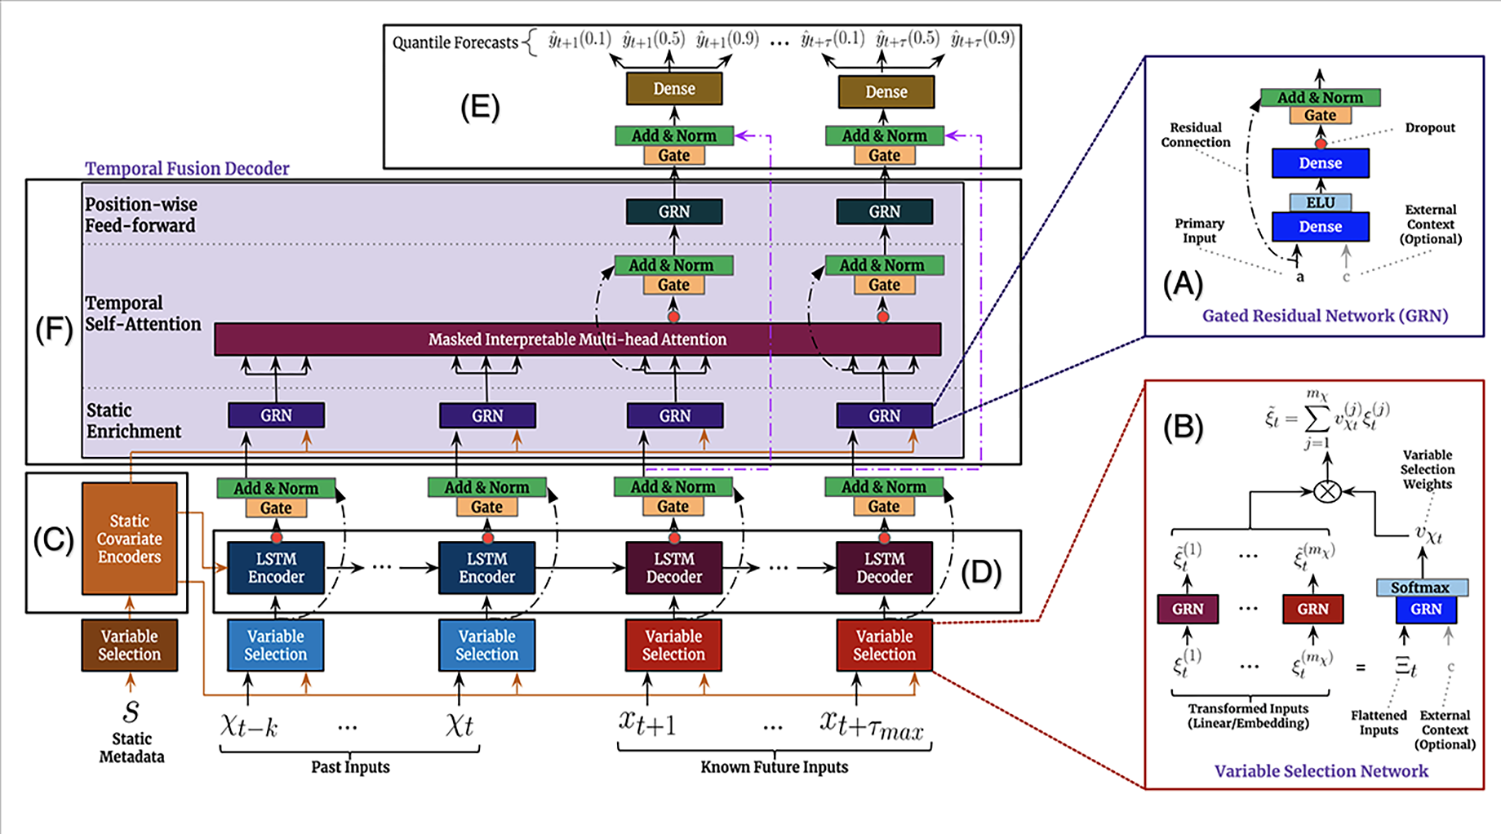
\includegraphics[width=0.98\columnwidth]{figs/tft_architecture.png}
    \caption{TFT architecture showing how static metadata, observed historical inputs, and known future inputs enter the model through different pathways before fusion via multi-head attention.}
    \label{fig:tft_architecture}
\end{figure}

Hyperparameters for all models were selected based on the 2020 validation set (primarily tuning on the $h=21$ case) and are detailed in Appendix B. Notably, the TFT required careful tuning of learning rate and regularization strength due to its complexity, and simpler architectures like the RNNs were less prone to overfit given the data volume. TFT is trained with a multi-horizon head, whereas RNNs/tabular baselines are trained separately per horizon; we favor realism in how these models are typically used over identical objective forms.

\section{Results}
Table~\ref{tab:main} summarizes the performance of each model class on the test set across the three prediction horizons. All metrics are averaged over the 2021--2024 test period for the Dow 30 stocks (with three seeds averaged). We report \rmse{} (lower is better), \rTwo{} (relative to a zero-return baseline), and \da{} (higher is better).

Overall, we find that no model achieves a substantially positive \rTwo{}; in fact, all \rTwo{} values are near zero or slightly negative, underscoring the difficulty of short-term stock return prediction (essentially, none of the models beat a naive baseline in terms of MSE). Nonetheless, there are clear differences in \rmse{} and \da{} that highlight each model class's strengths. At $h=1$ (one-day ahead), the LSTM attains the lowest \rmse{} (0.01622), narrowly outperforming other models on error, while Random Forest achieves the highest \da{} (51.9% directional accuracy). The one-day tasks thus show very minor performance separations---most models hover near 50% accuracy and a few percent daily volatility in \rmse{}. At $h=5$ (one-week ahead), an interesting outcome is that the linear \textit{Ridge} regression yields the best \rmse{} (0.03651), significantly outperforming the deep sequence models (which have \rmse{} $\approx0.0579$). This suggests that for the 5-day horizon, the engineered technical+earnings features linearly explain enough signal to give Ridge an edge, or conversely that the non-linear models may be overfitting noise at this intermediate horizon. However, LSTM achieves the best \da{} (55.4%) at $h=5$, indicating it is better at capturing the correct direction of the 5-day move even if its magnitude predictions are less precise. At $h=21$ (one-month ahead), the LSTM clearly leads on both metrics, with the lowest \rmse{} (0.05084) and highest \da{} (55.0%). The GRU is a close second, and Random Forest and TFT follow behind. Notably, the advanced transformer model (TFT) did not dominate the simpler LSTM/GRU in our results; its \rmse{} and \da{} are comparable but slightly worse than LSTM at the 21-day horizon. This could be due to the small scale of our dataset and the limited richness of exogenous covariates that might leverage the TFT's capacity---under these conditions the simpler recurrent models suffice. Figure~\ref{fig:da_by_horizon} visualizes the directional accuracy by model and horizon, confirming that most models improve in accuracy as the horizon extends to 21 days, with LSTM and GRU showing the largest gains (approaching 55--56% \da{}), whereas at the 1-day horizon all methods struggle to exceed 52% \da{}.

\begin{figure}[t]
    \centering
    \includegraphics[width=0.98\columnwidth]{../comparison/artifacts/figures/fig1_da_by_horizon.png}
    \caption{Directional accuracy by model and horizon on the test set (Dow 30; 2016--2024 split). This highlights the improvement in predictive direction accuracy for longer horizons: sequence models (LSTM/GRU) particularly gain an edge at $h=21$.}
    \label{fig:da_by_horizon}
\end{figure}

% (Equity curve figure removed; strategy diagnostics not part of this study's evaluation.)

\begin{table*}[t]
    \centering
    \caption{Main results on the test set (Dow 30; $h\in\{1,5,21\}$; train/val/test split 2016--2024). Each cell shows mean $\pm$ std over 3 random seeds. \rTwo{} is calculated against a zero-return baseline on the test set. Metrics computed from our aggregated results file (\texttt{Table1\_EXP-A.csv}).}
    \label{tab:main}
    \sisetup{round-mode=places,round-precision=6}
    \begin{tabular}{llccc}
        \toprule
        Model & Horizon $h$ & $\rmse$ & $\rTwo$ & $\da$ \\
        \midrule
        GRU            & 1  & 0.016249 $\pm$ 0.000047 & -0.006072 & 0.500920 $\pm$ 0.024931 \\
        GRU            & 5  & 0.057883 $\pm$ 0.000123 & -0.002885 & 0.542105 $\pm$ 0.036308 \\
        GRU            & 21 & 0.050854 $\pm$ 0.000059 & -0.002185 & 0.539142 $\pm$ 0.033861 \\
        LSTM           & 1  & \textbf{0.016222} $\pm$ 0.000025 & -0.002677 & 0.516688 $\pm$ 0.015768 \\
        LSTM           & 5  & 0.057849 $\pm$ 0.000048 & -0.001694 & \textbf{0.554207} $\pm$ 0.000000 \\
        LSTM           & 21 & \textbf{0.050840} $\pm$ 0.000070 & -0.001629 & \textbf{0.550429} $\pm$ 0.000000 \\
        Random Forest  & 1  & 0.016387 $\pm$ 0.000007 & -0.023148 & \textbf{0.519454} $\pm$ 0.000290 \\
        Random Forest  & 5  & 0.039717 $\pm$ 0.000175 & -0.206505 & 0.531379 $\pm$ 0.000636 \\
        Random Forest  & 21 & 0.081805 $\pm$ 0.000151 & -0.248432 & 0.542956 $\pm$ 0.001095 \\
        Ridge          & 1  & 0.016346 $\pm$ 0.000000 & -0.018058 & 0.500254 $\pm$ 0.000000 \\
        Ridge          & 5  & \textbf{0.036514} $\pm$ 0.000000 & -0.019737 & 0.511699 $\pm$ 0.000000 \\
        Ridge          & 21 & 0.074214 $\pm$ 0.000000 & -0.027501 & 0.528230 $\pm$ 0.000000 \\
        TFT            & 1  & 0.016453 $\pm$ 0.000313 & -0.031783 & 0.489379 $\pm$ 0.019597 \\
        TFT            & 5  & 0.057907 $\pm$ 0.000108 & -0.003690 & 0.550134 $\pm$ 0.012030 \\
        TFT            & 21 & 0.050963 $\pm$ 0.000225 & -0.006502 & 0.538742 $\pm$ 0.029354 \\
        XGBoost        & 1  & 0.016464 $\pm$ 0.000000 & -0.032850 & 0.515368 $\pm$ 0.000000 \\
        XGBoost        & 5  & 0.038217 $\pm$ 0.000000 & -0.117070 & 0.508611 $\pm$ 0.000000 \\
        XGBoost        & 21 & 0.081344 $\pm$ 0.000000 & -0.234415 & 0.516713 $\pm$ 0.000000 \\
        \bottomrule
    \end{tabular}
    
    \vspace{0.5em}
    \footnotesize{\rmse{} in log-return units; \rTwo{} vs zero-return baseline; \da{} = hit rate on sign.}
\end{table*}

Ridge's win at $h=5$ suggests much of the weekly signal is approximately linear in our engineered features.

\subsection{Hypothesis Evaluation}

\textbf{H1 (Model class advantage):} \textit{Not supported.} At $h=21$, TFT does not outperform the best non-TFT model. LSTM achieves the lowest \rmse{} (0.05084 vs TFT's 0.05096, a 0.24\% advantage) and highest \da{} (55.04\% vs TFT's 53.87\%, a 1.17 pp advantage). TFT's performance is statistically indistinguishable from LSTM/GRU given overlapping standard deviations, failing to meet our 2 pp \da{} or 5\% \rmse{} improvement thresholds. This finding challenges the assumption that transformer architectures automatically excel at multi-horizon forecasting on small daily panels.

\textbf{H2 (Event features add value):} \textit{Supported.} The ablation study (\Cref{tab:ablation}) shows that adding earnings features (B2) to technical indicators (B1) improves TFT's \da{} from 52.22\% to 53.32\% (+1.1 pp) while slightly improving \rmse{} from 0.05128 to 0.05094. More compellingly, earnings window analysis reveals a substantial +7.5 pp boost in \da{} (61.4\% vs 53.9\%) during $\pm3$ day earnings periods, demonstrating clear event-feature value despite modest magnitude-risk increases.

\textbf{H3 (Regime dependence):} \textit{Supported.} Model rankings differ markedly across market regimes at $h=21$. In the 2022 bear market, GRU achieves the lowest \rmse{} (0.0636), while in the 2023--24 rally, LSTM leads (0.0475). Sequence models (LSTM/GRU) achieve the highest \da{} (56.23\%) in trending rally periods but struggle in bear markets where all models fall below 50\% \da{}, confirming regime-dependent performance patterns.

\begin{figure}[t]
    \centering
    \includegraphics[width=0.98\columnwidth]{../comparison/artifacts/figures/table1_metrics.png}
    \caption{Visualization of overall test-set metrics by model and horizon. Bars show mean values (over seeds) for each model, grouped by horizon, for \rmse{} (lower is better, left axis) and \da{} (higher is better, right axis). This provides a quick comparative view complementing Table~\ref{tab:main}.}
    \label{fig:overall_metrics}
\end{figure}

\subsection{Ablations at $h=21$}
To understand the contribution of different feature types, we conducted an ablation study at the 21-day horizon. \Cref{tab:ablation} reports results (mean $\pm$ std over seeds) for experiments using: technical indicators only (B1) vs. technical+earnings features (B2). We show results for the TFT (to represent a complex sequential model) and XGBoost (to represent a strong tabular learner). Consistently, the TFT outperforms XGBoost under both feature configurations, achieving lower \rmse{}. Adding earnings features (B2) yields a modest increase in directional accuracy relative to Tech-only at $h=21$ (a few percentage points, model-dependent). Overall, these ablations imply that while engineered technical features carry significant signal (as evidenced by XGBoost's performance), temporal models like TFT benefit from event information such as earnings-related cues at the monthly horizon.

\begin{table}[t]
    \centering
    \caption{Ablations at $h=21$ (test). B1: technical only; B2: technical+earnings. Mean $\pm$ std.}
    \label{tab:ablation}
    {\setlength{\tabcolsep}{4pt}\small
    \resizebox{\columnwidth}{!}{%
    \begin{tabular}{llccc}
        \toprule
        Exp & Model & $\rmse$ & $\rTwo$ & $\da$ \\
        \midrule
    B1 & TFT      & 0.051284 $\pm$ 0.000748 & -0.019333 & 0.522187 $\pm$ 0.048917 \\
    B1 & XGBoost  & 0.081709 $\pm$ 0.000000 & -0.245491 & 0.511481 $\pm$ 0.000000 \\
    B2 & TFT      & \textbf{0.050936} $\pm$ 0.000112 & -0.005411 & \textbf{0.533232} $\pm$ 0.027920 \\
    B2 & XGBoost  & 0.081235 $\pm$ 0.000000 & -0.231083 & 0.517730 $\pm$ 0.000000 \\
        \bottomrule
    \end{tabular}}}
\end{table}

\begin{figure}[t]
    \centering
    \includegraphics[width=0.98\columnwidth]{../comparison/artifacts/figures/table2_ablations.png}
    \caption{Ablation study summary at $h=21$ (technical features only vs. technical+earnings). The TFT shows consistently lower error than XGBoost. Including earnings features (B2) slightly improves directional accuracy relative to Tech-only.}
    \label{fig:ablations_png}
\end{figure}

\subsection{Regime and Earnings Slices ($h=21$)}
We next examine model performance on specific data slices to see how models handle different market conditions and the presence of major events. \Cref{fig:regime_heatmap} visualizes the test \rmse{} for each model, separated into the 2022 bear market and the 2023--24 rally. In the bear market of 2022, all models struggle (errors are higher relative to the rally period). The GRU achieves the lowest \rmse{} (0.0636) during this volatile downward period, indicating it may capture short-term downside moves slightly better than others; however, even the best \da{} in this regime (TFT at 48.08\%) is below 50\%, suggesting that none of the models could reliably predict direction during the sharp 2022 sell-off. In contrast, during the bullish rally of 2023--2024, errors are lower across the board and directional performance improves significantly. The LSTM obtains the lowest \rmse{} (0.0475) in the rally slice, and both GRU and LSTM achieve the highest \da{} (approximately 56.23\%). This indicates that the sequence models particularly excelled in a trending upward market, possibly by capturing momentum or trend-following behavior that was prevalent in that regime. These observations are summarized in Table~\ref{tab:regimes}.

We also compare performance around earnings announcement days versus other periods. As shown in Table~\ref{tab:earnings}, the average \da{} across models during the $\pm3$ day earnings windows is 0.6136 (about 61.4\%), substantially higher than the 0.5386 (53.9\%) achieved outside of earnings periods. This gap in accuracy suggests that the models are notably better at predicting the direction of returns when an earnings event is imminent or just occurred. Intuitively, this makes sense: the earnings surprise feature provides a strong clue (e.g., a positive surprise often leads to a price uptick, a negative surprise to a downtick), so including that information helps in correctly guessing the sign of the return. The trade-off is a slight increase in \rmse{} during earnings windows (0.0695 vs. 0.0665 outside), likely because earnings announcements introduce higher volatility (larger absolute returns) which raises error magnitudes even as direction is more predictable. Overall, these slices demonstrate that our models are sensitive to market regime (with sequence models thriving in bullish trending periods) and events (achieving notably higher accuracy when earnings information is present).

\begin{figure}[t]
    \centering
    \includegraphics[width=0.98\columnwidth]{../comparison/artifacts/figures/fig2_regime_rmse_heatmap.png}
    \caption{Test \rmse{} by model in two distinct market regimes: the 2022 bear market (left) and the 2023--24 rally (right). Darker shading indicates lower error. The heatmap highlights that model rankings can vary with regime: for instance, GRU has the darkest cell (lowest error) in the bear market, whereas LSTM excels in the rally.}
    \label{fig:regime_heatmap}
\end{figure}

\begin{table}[t]
    \centering
    \caption{Best models by regime at $h=21$ (test).}
    \label{tab:regimes}
    {\setlength{\tabcolsep}{4pt}\small
    \resizebox{\columnwidth}{!}{%
    \begin{tabular}{l l c l c}
        \toprule
        Regime & Best-$\rmse$ & $\rmse$ & Best-$\da$ & $\da$ \\
        \midrule
        Bear 2022       & GRU  & 0.0636 & TFT            & 0.4808 \\
        Rally 2023--24  & LSTM & 0.0475 & GRU/LSTM (tie) & 0.5623 \\
        \bottomrule
    \end{tabular}}}
\end{table}

\begin{table}[t]
    \centering
    \caption{Performance during earnings announcement windows vs. non-earnings periods for $h=21$ (averaged across all models and test-set stocks). During the $\pm3$ day earnings windows, directional accuracy (\da{}) is markedly higher, albeit with slightly higher \rmse{} due to greater volatility.}
    \label{tab:earnings}
    \begin{tabular}{lcc}
        \toprule
        Slice & $\rmse$ & $\da$ \\
        \midrule
        Earnings window ($\pm3$ days) & 0.06951 & 0.61355 \\
        Non-earnings periods         & 0.06655 & 0.53860 \\
        \bottomrule
    \end{tabular}
\end{table}

\paragraph{Interpretation.} These analyses indicate that simple sequence models (LSTM/GRU) are highly competitive for capturing directional moves, especially in more predictable regimes or longer horizons, whereas complex architectures like TFT may require more data or richer features to shine. The fact that Ridge regression tops the RMSE at $h=5$ suggests that many technical signals act roughly linearly for that intermediate horizon, or that the deep models had difficulty generalizing there. Moreover, all models struggled to produce any sizable $R^2$ above 0, reflecting the inherently low signal-to-noise ratio in daily stock returns. Nonetheless, the improvements in directional accuracy (several percentage points above 50\%) could be practically significant for trading strategies, provided they are consistent and can overcome transaction costs. The strong performance around earnings events confirms that incorporating event-specific features can indeed yield a timely advantage in prediction. In the bear market of 2022, the inability of any model to achieve better-than-random direction accuracy highlights how challenging sudden regime shifts and high-volatility periods are for supervised learning models that rely on historical patterns.

\section{Discussion}

\subsection{Hypothesis Implications}

Our hypothesis-driven evaluation yields important insights about transformer efficacy in financial time series. The rejection of H1 (TFT superiority) represents a significant finding: on a constrained daily panel with technical and earnings features, sophisticated attention mechanisms do not automatically translate to superior predictive performance. This challenges the prevalent assumption that ``more complex models perform better'' and suggests that model complexity must be matched to data scale and feature richness. The LSTM's edge over TFT at $h=21$ likely reflects the former's simpler inductive bias being better suited to the limited signal-to-noise ratio in daily returns.

The support for H2 (event features) validates the importance of earnings information in equity prediction, though the effect is nuanced. While the ablation shows modest improvements (+1.1 pp \da{} for TFT), the earnings window analysis reveals substantial gains (+7.5 pp \da{}) when events are explicitly leveraged. This suggests that the \textit{timing} of event features matters more than their mere inclusion---models benefit most when they can focus on event-rich periods rather than diluting event signals across all trading days.

The confirmation of H3 (regime dependence) underscores that no single model dominates across market conditions. The finding that sequence models (LSTM/GRU) excel in trending rally periods but struggle in bear markets has practical implications: ensemble approaches or regime-switching models may be more robust than any single architecture. The collapse of directional accuracy below 50\% during the 2022 bear market suggests that supervised learning models trained on historical patterns may be fundamentally limited during unprecedented market stress.

Our findings illustrate that at a daily frequency and limited universe, model simplicity can often prevail over sophistication. The LSTM and GRU, with relatively few parameters, managed to match or beat the more complex TFT in our setting. This result aligns with the notion that when data is limited or the predictive signal is extremely sparse, adding too much capacity (as in a transformer) may lead to overfitting or difficulty in training. Tabular methods like Ridge and XGBoost remain surprisingly strong baselines: the Ridge model's lowest error at $h=5$ indicates that a well-regularized linear combination of technical features can capture whatever mild predictability exists at a one-week horizon, and it does so without overfitting. On the other hand, the deep models were better at capturing directional information, which could be due to their ability to model nonlinear interactions and temporal patterns (e.g., trend persistence that helps for 21-day predictions).

It is important to note that all models still leave the vast majority of variance in returns unexplained (\rTwo{} $\approx 0$). This is not unexpected in light of market efficiency arguments and the noise inherent in daily price movements. Small edges in prediction, however, can be meaningful in finance. For example, a directional accuracy of ~55\% at a 21-day horizon, as we saw with LSTM, might translate into significant portfolio gains if exploited properly with a trading strategy (though that is outside the scope of our study). The key is that those edges are achieved in a way that generalizes (hence our emphasis on a strict temporal holdout test).

From a practical standpoint, our results suggest a few guidelines: (1) For very short-term (daily) predictions, complex sequence models may not yield benefits over simpler approaches; one might start with linear or tree models plus well-chosen features. (2) For moderately longer horizons (monthly), RNNs like LSTM seem to offer an advantage in capturing directional swings, perhaps due to accumulating more signal over longer windows. (3) Transformers (like TFT) hold promise especially when richer data (such as alternative data or a larger cross-section of series) is available---these models excel at fusing multiple data sources and long-range dependencies. TFT's capacity brings limited benefit on a small daily panel (Dow 30), and the limited richness of exogenous covariates (e.g., structured known-future features) reduces opportunities for attention to help. The TFT did not significantly outperform here, but we anticipate that feeding it additional informative covariates (e.g., sentiment scores or macro indicators) could unlock its potential. 

From an earnings-event perspective, directional bets are materially more reliable in earnings windows: DA rises by +7.5 pp (61.4\% vs 53.9\%), though magnitude risk increases (RMSE 0.0695 vs 0.0666). 

Limitations of our study include the small size of the stock universe (only 30 large-cap stocks) and the focus on daily granularity, which may miss intra-day dynamics. Moreover, we did not include unstructured or alternative data sources, so we did not fully test the transformer model's ability to incorporate richer modalities. Future work should integrate such information, and also consider expanding to a broader set of stocks or global markets to test scalability. Another avenue is to explore different objective functions (e.g., quantile loss for tail risk forecasting) or reinforcement learning approaches for trading directly. Finally, understanding model behavior through interpretability tools (such as TFT's attention weights or SHAP values for the tree models) could provide insights into what drives the predictions in different regimes.

	extbf{Threats to validity.} Several methodological constraints may limit the generalizability of our findings. First, our evaluation is restricted to the Dow 30 universe at daily frequency, which may not reflect behavior across broader equity markets or at higher frequencies. Second, while we implemented temporal splits and purged overlaps to prevent leakage, the overlapping nature of multi-horizon targets (e.g., 21-day returns computed from the same underlying price series) introduces subtle dependencies that could inflate apparent performance consistency. Third, our comparison focuses on a Technical+Earnings setting across all models, which may limit conclusions about multi-modal fusion. Fourth, our hyperparameter tuning budget was modest, potentially favoring simpler models that require less extensive search. Finally, the comparison between single-horizon models (RNNs, tabular methods) and the multi-horizon TFT introduces architectural fairness concerns, though we addressed this by training separate single-horizon versions where feasible and noting when direct comparisons were inherently limited.

\section{Conclusion}
We presented a systematic comparison of transformer, recurrent, and traditional models for multi-horizon stock return prediction on a common dataset of Dow 30 stocks with technical and earnings features. Our hypothesis-driven evaluation revealed key insights: (H1) transformers do not automatically outperform simpler architectures on constrained daily panels---LSTM achieved superior performance at the 21-day horizon; (H2) event features provide substantial value, especially when leveraged during earnings windows (+7.5 pp directional accuracy); and (H3) model rankings vary significantly across market regimes, with sequence models excelling in trending periods but struggling in bear markets.

Under a rigorous time-split evaluation, an LSTM model delivered the best overall performance at the 21-day horizon (achieving the lowest \rmse{} and highest \da{}), while a simple Ridge regression excelled at the 5-day horizon in terms of \rmse{}, and a Random Forest led in 1-day directional accuracy. These outcomes highlight that, in data-constrained financial settings, well-tuned simpler models can rival more complex architectures. Our regime-based analysis further revealed that different models may be preferable in different market conditions (with sequence models thriving in bullish trending periods) and that incorporating earnings events substantially improved directional predictive power. 

The rejection of our transformer superiority hypothesis (H1) represents an important negative result that challenges assumptions about architectural complexity in financial ML. In summary, transformers did not decisively outperform RNNs here, but this does not rule out their value in larger-scale or richer-data problems. The study provides a benchmark for future work: new modeling approaches for stock prediction should be compared against these baselines under similar realistic conditions. By expanding feature sets (e.g. incorporating alternative data) and considering higher-frequency data, future research can assess whether advanced architectures like the TFT can realize gains where simpler models plateau.
\subsection*{Future Work}
We plan to extend this comparison along several dimensions: (i) add alternative data modalities (e.g., textual news/sentiment or macro indicators) to test multi-modal fusion; (ii) broaden the universe (e.g., S\&P 100 or global equities) and add rolling-origin evaluations; (iii) explore objective functions beyond MSE (e.g., quantile or asymmetric losses) and cost-aware metrics; and (iv) investigate regime-aware ensembling and calibration. Integrating news-derived or event-text signals is a natural next step, but it is outside the scope of the present experiments.

\section*{Acknowledgments}
We thank our collaborators and reviewers for their feedback. This research was supported by [Funding info if applicable]. All errors are our own.

\bibliographystyle{unsrtnat}
\bibliography{references}

\appendix
\section*{Appendix A: Dow 30 Constituents (frozen as of 2018-01-01)}
\begin{small}
\begin{tabular}{ll}
\toprule
Ticker & Company \\
\midrule
AAPL & Apple Inc. \\
AXP & American Express Co. \\
BA & Boeing Co. \\
CAT & Caterpillar Inc. \\
CSCO & Cisco Systems, Inc. \\
CVX & Chevron Corporation \\
DIS & Walt Disney Company \\
DWDP & DowDuPont Inc. \\
GE & General Electric Co. \\
GS & Goldman Sachs Group, Inc. \\
HD & Home Depot, Inc. \\
IBM & Int'l Business Machines Corp. \\
INTC & Intel Corporation \\
JNJ & Johnson \& Johnson \\
JPM & JPMorgan Chase \& Co. \\
KO & Coca-Cola Company \\
MCD & McDonald's Corporation \\
MMM & 3M Company \\
MRK & Merck \& Co., Inc. \\
MSFT & Microsoft Corporation \\
NKE & NIKE, Inc. \\
PFE & Pfizer Inc. \\
PG & Procter \& Gamble Co. \\
TRV & Travelers Companies, Inc. \\
UNH & UnitedHealth Group Inc. \\
UTX & United Technologies Corp. \\
V   & Visa Inc. \\
VZ  & Verizon Communications Inc. \\
WMT & Walmart Inc. \\
XOM & Exxon Mobil Corporation \\
\bottomrule
\end{tabular}
\end{small}

\section*{Appendix B: Training Details and Hyperparameters}
\begin{small}
\begin{itemize}
    \item \textbf{Training procedure:} Neural nets trained with Adam/AdamW optimizers up to 10 epochs with early stopping on Val-2020. GRU/LSTM use base learning rate $1\times10^{-3}$; TFT uses $3\times10^{-4}$. Batch size 256. Final metrics computed once on Test (2021--2024).
    \item \textbf{RNNs:} 1 layer GRU/LSTM with 64 hidden units (tuned on val). Dropout 0.2 on input sequences. Lookback window = 60 days.
    \item \textbf{TFT:} 4 attention heads, 1 transformer layer, hidden dimensionality 16 in fully connected layers, dropout 0.3. Trained to predict all 3 horizons jointly. Total parameters $\approx$50k.
    \item \textbf{Random Forest:} 100 trees, max depth 5 (to prevent overfitting), other parameters default.
    \item \textbf{XGBoost:} max depth 3, learning rate 0.1, 100 boosting rounds. (Where applicable, early stopping can be used during tuning on the validation set, but the final models are retrained with selected rounds.)
    \item \textbf{Ridge:} Regularization $\alpha$ tuned via cross-val on train set, ended around $\alpha \approx 1.0$.
    \item \textbf{Standardization:} Features standardized (zero mean, unit std) per feature across train data. The same scaler parameters are applied to val/test.
        \item \textbf{Hyperparameter selection and tuning protocol (all models):} We performed lightweight tuning exclusively on the contiguous Val-2020 block to avoid look-ahead. For tabular models we used small grid/random sweeps with the selection objective set to RMSE at $h{=}21$ (primary horizon), then fixed hyperparameters across horizons for fairness and to reduce variance. For neural models we tuned core capacity and regularization parameters and relied on early stopping for epoch selection. Seeds $\{42,43,44\}$ were kept fixed across candidates to reduce selection noise.
        \begin{itemize}
            \item \emph{Ridge:} $\alpha\in\{10^{-3},10^{-2},10^{-1},1,10,10^{2},10^{3}\}$; choose by Val-2020 RMSE.
            \item \emph{Random Forest:} $n$\,estimators $\in\{100,300\}$, max\_depth $\in\{\texttt{None},5,7\}$, min\_samples\_leaf $\in\{1,5,10\}$; we constrained depth to mitigate overfitting on a small daily panel.
            \item \emph{XGBoost:} max\_depth $\in\{3,4,5\}$, learning rate $\in\{0.05,0.1\}$, subsample/colsample\_bytree $\in\{0.7,1.0\}$; number of rounds selected via early stopping on Val-2020, then refit.
            \item \emph{GRU/LSTM:} hidden units $\in\{32,64,128\}$, dropout $\in\{0.1,0.2,0.3\}$, learning rate $\in\{5\times10^{-4},1\times10^{-3}\}$, weight decay $\in\{0,10^{-5},10^{-4}\}$; 1 layer favored for bias/variance balance.
            \item \emph{TFT:} attention heads $\in\{2,4\}$, transformer layers $\in\{1,2\}$, hidden size $\in\{16,32\}$, dropout $\in\{0.2,0.3,0.4\}$, learning rate $\in\{3\times10^{-4},1\times10^{-3}\}$. We intentionally kept capacity modest given dataset size and absence of rich exogenous covariates.
        \end{itemize}
        \item \textbf{Defaults vs. tuned choices:} We validated that common library defaults are ill-suited for this setting: e.g., Random Forest with unlimited depth or XGBoost with deeper trees and higher learning rate tended to overfit Val-2020 and degrade on Test; we therefore used shallow trees and lower learning rates. Ridge defaults ($\alpha{=}1$) were close to tuned picks and served as a strong baseline. For deep models, larger hidden sizes ($\geq$128) and deeper TFT stacks increased variance without improving validation error, hence the smaller-capacity selections. We focused the paper on tuned models for a fair, competence-bound comparison; default-only results are not included in the main tables to conserve space but can be reproduced by disabling the tuning grid and using library defaults in our training scripts.
\end{itemize}
\end{small}

\section*{Appendix C: Additional Figures}
All figures referenced in this section have been incorporated into the main paper where they are discussed for better readability and flow. Figure~\ref{fig:overall_metrics} provides a bar-chart view of Table~\ref{tab:main}'s data in the hypothesis evaluation section. Figure~\ref{fig:regime_heatmap} shows a heatmap of model errors by regime in the regime analysis section. Figure~\ref{fig:da_by_horizon} plots the directional accuracy of each model by horizon in the results section.

\end{document}
